\documentclass[11pt,a4paper]{article}

% ---- Packages ----------------------------------------------------------
\usepackage[utf8]{inputenc}
\usepackage[T1]{fontenc}
\usepackage{lmodern}
\usepackage[margin=0.95in]{geometry}
\usepackage{microtype}
\usepackage{amsmath,amssymb}
\usepackage{titlesec}
\usepackage{enumitem}
\usepackage{booktabs}
\usepackage{array}
\usepackage{tabularx}
\usepackage{xcolor}
\usepackage{fancyhdr}
\usepackage{graphicx}
\usepackage{float}
\usepackage{caption}
\usepackage{subcaption}
\usepackage{tikz}
\usetikzlibrary{positioning,arrows.meta,shapes.geometric,backgrounds,fit,calc}
\usepackage[hidelinks,colorlinks=true,linkcolor=cool,citecolor=teal,urlcolor=teal]{hyperref}
\usepackage{parskip}

% ---- Colour palette ----------------------------------------------------
\definecolor{accent}{HTML}{0F766E}
\definecolor{cool}{HTML}{1E3A8A}
\definecolor{amber}{HTML}{D97706}
\definecolor{rose}{HTML}{BE123C}
\definecolor{neutral}{HTML}{475569}
\definecolor{panel}{HTML}{F1F5F9}
\definecolor{paneledge}{HTML}{CBD5E1}

% ---- Header / Footer ---------------------------------------------------
\pagestyle{fancy}
\fancyhf{}
\fancyhead[L]{\small\textcolor{neutral}{Flow-Pattern Anomaly Detection at the IoT Gateway}}
\fancyhead[R]{\small\textcolor{neutral}{Madhav Dogra}}
\fancyfoot[C]{\small\thepage}
\renewcommand{\headrulewidth}{0.4pt}
\renewcommand{\headrule}{\hbox to\headwidth{\color{paneledge}\leaders\hrule height \headrulewidth\hfill}}

% ---- Section formatting ------------------------------------------------
\titleformat{\section}{\normalfont\large\bfseries\color{cool}}{\thesection}{0.6em}{}
\titleformat{\subsection}{\normalfont\normalsize\bfseries\color{accent}}{\thesubsection}{0.5em}{}
\titlespacing*{\section}{0pt}{12pt}{4pt}
\titlespacing*{\subsection}{0pt}{8pt}{2pt}
\setlength{\parskip}{4pt}
\newcommand{\hd}[1]{\textbf{\textcolor{accent}{#1}}}
\captionsetup{font=small,labelfont={bf,color=cool},skip=4pt}

% ---- Callout box -------------------------------------------------------
\newcommand{\keybox}[2]{%
\begin{tikzpicture}
\node[fill=panel,draw=paneledge,rounded corners=3pt,inner sep=8pt,text width=\dimexpr\linewidth-20pt\relax] {%
\textbf{\textcolor{accent}{#1}}\ \ #2};
\end{tikzpicture}}

% =======================================================================
\begin{document}

% ---- Title block -------------------------------------------------------
\begin{titlepage}
\centering
\vspace*{1.1cm}
{\large\textcolor{neutral}{Scientific Analysis Group (SAG), DRDO}}\\[0.25cm]
{\small\textcolor{neutral}{Internship Progress Report}}\\[0.9cm]
{\color{cool}\rule{\linewidth}{1.4pt}}\\[0.5cm]
{\LARGE\bfseries\color{cool} Flow-Pattern Anomaly Detection\\[5pt] at the IoT Gateway}\\[0.55cm]
{\large\itshape A Pre-trained Mamba Detector for Known and Zero-Day Attacks}\\[0.4cm]
{\color{cool}\rule{\linewidth}{0.7pt}}\\[1.5cm]
{\Large\textbf{Madhav Dogra}}\\[1.7cm]
{\renewcommand{\arraystretch}{1.5}
\begin{tabular}{@{}r@{\quad}l@{}}
\textcolor{accent}{\textbf{Department}} & Computer Science \& Engineering \\
\textcolor{accent}{\textbf{Date of Joining (DOJ)}} & 11\textsuperscript{th} May 2026 \\
\textcolor{accent}{\textbf{Internship Duration}} & 8 Weeks \\
\textcolor{accent}{\textbf{Mentor}} & Sh Sankalp Kumar Gupta, Sc `E', SAG \\
\end{tabular}\par}
\vfill
{\small\textcolor{neutral}{\texttt{flowmamba} prototype \;$\cdot$\; IoT-23 real malware traffic \;$\cdot$\; CPU (Apple M3 Pro)}}\\[0.4cm]
{\small\textcolor{neutral}{2026-07-03}}
\end{titlepage}

\begin{abstract}
\noindent
IoT gateways see every device flow but cannot host endpoint security agents, so
attack detection must happen \emph{on the network}, cheaply, and on encrypted
traffic. This report documents \texttt{flowmamba}, a lightweight detector that
keeps the \emph{packet order} of a connection --- the first $K$ packets as an
ordered sequence of payload-free features --- and feeds it to a shared Mamba
state-space encoder with two heads: a supervised classifier for known attacks
and a one-class deep-SVDD scorer for zero-days. We trace the empirical journey
from a single-capture prototype (macro-F1 0.79, anomaly ROC-AUC 0.994) to a
multi-source model trained on seven IoT-23 captures. The central practical
finding is that, with payload-free features on \emph{short} flows, the model
separates traffic by \textbf{flow structure} --- benign vs.\ short scan/botnet
attacks vs.\ long brute-force --- but \emph{not} by fine attack family (DDoS,
Recon and Mirai-C\&C are inseparable in the first few packets, proven three
independent ways). Aligning the label taxonomy with what the features can
actually resolve yields a clean three-class detector at \textbf{98.2\,\%
accuracy}, macro-F1 \textbf{0.984}, anomaly ROC-AUC \textbf{0.935}, and
$\sim$5\,ms/flow latency. We close with the open question a CNN sub-classifier
is meant to test.
\end{abstract}

\vspace{2pt}
\noindent\keybox{Headline.}{Final three-class model --- \textbf{98.2\,\% accuracy},
macro-F1 \textbf{0.984}, anomaly ROC-AUC \textbf{0.935}, 5.0\,ms/flow --- trained
on seven real IoT-23 malware captures. The accuracy ceiling is set by genuine
feature overlap among short-flow attack families, not by model capacity.}

% =======================================================================
\section{Motivation}

The target environment is the modern smart home, escalating to a defence
context: \emph{``field sensors, surveillance equipment and base infrastructure
are high-value, low-trust devices that cannot be hardened one by one.''} IoT
devices ship with default credentials, run rarely-updated firmware, and lack the
compute to host any endpoint agent --- the Mirai botnet, built from compromised
IP cameras and routers, is the canonical proof this surface is exploitable at
scale. IoT anomaly detection at large is surveyed in~\cite{morshedi,survey23}.

Since software cannot sit \emph{on} the devices, the detector watches them
\emph{on the network}. The gateway is the single point through which every
device flow passes, and the only place modern compute can sit without
instrumenting the fleet. That vantage comes with one hard constraint that shapes
every design choice: gateway hardware is Raspberry-Pi-class, so the detector must
be small and fast --- a target of \textbf{$<$10\,ms per flow}.

\noindent A useful gateway detector must do four things at once:
\begin{enumerate}[leftmargin=1.4em,itemsep=1pt,topsep=2pt]
\item \hd{Catch known attacks} with high precision (supervised classifier).
\item \hd{Catch unknown, zero-day attacks} --- learn ``normal'' and flag whatever
does not fit, \emph{without ever training on the attack} (one-class anomaly head).
\item \hd{Work on encrypted traffic} --- read flow metadata only, never payload.
\item \hd{Run at the gateway} on small hardware, under 10\,ms per flow.
\end{enumerate}

% =======================================================================
\section{Related Work}

IoT anomaly detection is a crowded field; recent surveys map the
landscape~\cite{morshedi,survey23}. Four families are relevant here, and each
meets only part of the gateway brief (Table~\ref{tab:related}).

\hd{Signature / firewall} rules catch known attacks precisely but miss zero-days
and rely on deep packet inspection, which encryption defeats. \hd{Flow-statistic
ML} (XGBoost, random forests on $\approx$80 aggregate features) is cheap and
edge-friendly but \emph{order-agnostic} --- it discards the packet-sequence
structure that attack signatures live in. \hd{Pre-trained transformers}
(ET-BERT~\cite{etbert}) reach state-of-the-art accuracy on encrypted traffic but
at $\sim$110M parameters do not fit gateway hardware; even purpose-built
transformer studies for constrained IoT report this
tension~\cite{transformeriot}. \hd{One-class / autoencoder} detectors catch
novelty but cannot name known-attack categories.

Our design follows NetMamba~\cite{netmamba}: a selective state-space encoder that
keeps transformer-class accuracy at edge cost, extended with a \emph{shared
encoder $+$ dual head} so one representation serves both known-attack
classification and zero-day anomaly scoring. Complementary directions --- graph
IDS (E-GraphSAGE~\cite{egraphsage}), federated training across
sites~\cite{flids,peiotds}, and explainable zero-day alerts~\cite{xai} --- are
noted as future extensions.

\begin{table}[H]
\centering\small
\caption{Where existing approaches meet the four gateway requirements.}
\label{tab:related}
\renewcommand{\arraystretch}{1.2}
\begin{tabularx}{\linewidth}{@{}Xcccc@{}}
\toprule
\textbf{Approach} & \textbf{Known} & \textbf{Zero-day} & \textbf{Encrypted} & \textbf{Edge} \\
\midrule
Signature / firewall                 & \checkmark & --- & --- & \checkmark \\
Flow-statistic ML (XGBoost)          & \checkmark & $\sim$ & \checkmark & \checkmark \\
Transformer (ET-BERT)                & \checkmark & $\sim$ & \checkmark & --- \\
One-class / autoencoder              & --- & \checkmark & \checkmark & $\sim$ \\
\textbf{This work (Mamba dual-head)} & \checkmark & \checkmark & \checkmark & \checkmark \\
\bottomrule
\end{tabularx}
\end{table}

% =======================================================================
\section{Approach and Architecture}

\subsection{The representational bet: keep the order}
Conventional IDS collapses a flow into $\sim$80 summary statistics --- convenient
but \emph{permutation-invariant}: shuffle the packets and the statistics do not
change, destroying the temporal structure attack signatures live in. The core
bet of this work is the opposite: \textbf{keep the order}. A flow is the first
$K\!\approx\!32$ packets of a connection, kept as an ordered sequence
$x=(p_1,\dots,p_K)$, each packet described by a $13$-dimensional payload-free
vector (Table~\ref{tab:feat}). Because the features are header/metadata only, the
representation works on encrypted traffic.

\begin{table}[H]
\centering\small
\caption{The 13 payload-free per-packet features (\texttt{flowmamba.data.features}).}
\label{tab:feat}
\renewcommand{\arraystretch}{1.1}
\begin{tabularx}{\linewidth}{@{}p{0.16\linewidth}X@{}}
\toprule
\textbf{Group} & \textbf{Features} \\
\midrule
Size / timing & \texttt{size} (bytes), \texttt{iat} (inter-arrival time), \texttt{header\_len} \\
Direction     & \texttt{direction} ($+1$ up / $-1$ down) \\
TCP flags     & \texttt{syn}, \texttt{ack}, \texttt{fin}, \texttt{rst}, \texttt{psh}, \texttt{urg} \\
Header fields & \texttt{ttl}, \texttt{win} (TCP window), \texttt{is\_tcp} \\
\bottomrule
\end{tabularx}
\end{table}

\subsection{Why Mamba, and the shared-encoder design}
The reference pre-trained traffic detector, ET-BERT~\cite{etbert}, is a $\sim$110M-parameter
transformer that does not fit on a Raspberry Pi~\cite{transformeriot}. NetMamba~\cite{netmamba} showed a Mamba~\cite{mamba}
state-space model reaches comparable accuracy at far lower parameter and latency
cost --- Mamba is $O(K)$ in sequence length with $O(1)$ inference memory, versus
attention's $O(K^2)$; the selective state-space lineage runs from S4D~\cite{s4d}
through Mamba to Mamba-2~\cite{mamba2}. A \emph{single} encoder is shared by both heads
(Fig.~\ref{fig:arch}): pre-training is the expensive part, so sharing pays it
once, and it hands the anomaly head a representation of ``normal'' learned from a
large benign corpus --- exactly what a one-class scorer needs. The guiding
principle: \emph{``what's normal'' lives in the expensive encoder; ``what's
malicious'' lives in the cheap heads.}

% ---- Architecture diagram ----
\begin{figure}[H]
\centering
\resizebox{\linewidth}{!}{%
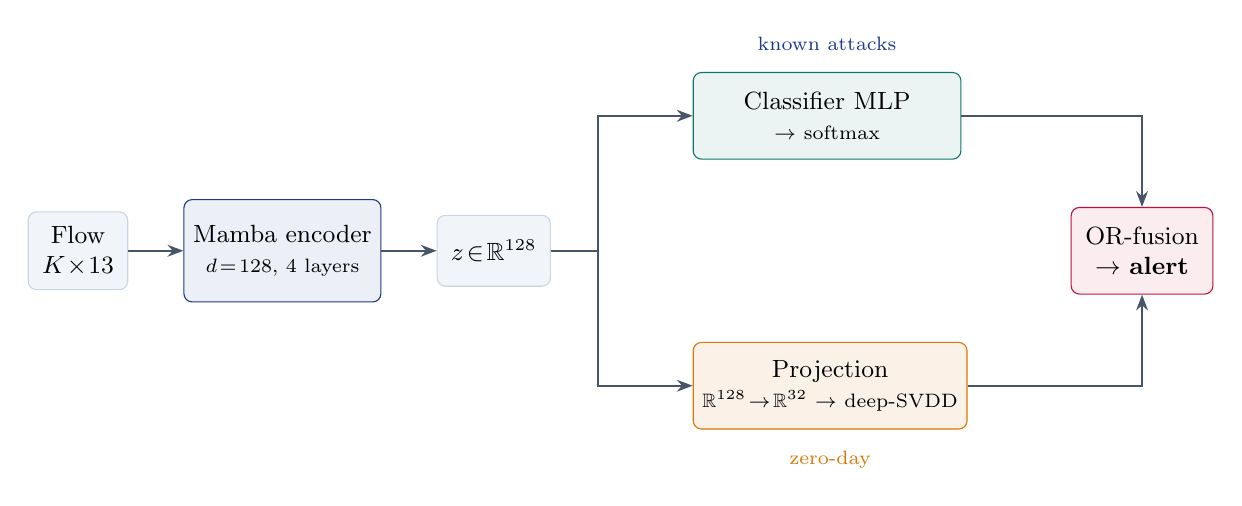
\begin{tikzpicture}[
  font=\small,
  box/.style={draw=paneledge,fill=panel,rounded corners=3pt,minimum height=9mm,inner sep=5pt,align=center},
  enc/.style={draw=cool,fill=cool!8,rounded corners=3pt,minimum height=13mm,minimum width=24mm,align=center},
  head/.style={draw=accent,fill=accent!8,rounded corners=3pt,minimum height=11mm,minimum width=34mm,align=center},
  ah/.style={draw=amber,fill=amber!10,rounded corners=3pt,minimum height=11mm,minimum width=34mm,align=center},
  fuse/.style={draw=rose,fill=rose!8,rounded corners=3pt,minimum height=11mm,minimum width=18mm,align=center},
  arr/.style={-{Stealth[length=2mm]},thick,neutral}
]
\node[box] (in) {Flow\\$K\!\times\!13$};
\node[enc,right=7mm of in] (enc) {Mamba encoder\\{\scriptsize $d\!=\!128$, 4 layers}};
\node[box,right=7mm of enc] (z) {$z\!\in\!\mathbb{R}^{128}$};
\node[head,above right=7mm and 18mm of z] (cls) {Classifier MLP\\{\scriptsize $\rightarrow$ softmax}};
\node[ah,below right=7mm and 18mm of z] (proj) {Projection\\{\scriptsize $\mathbb{R}^{128}\!\to\!\mathbb{R}^{32}$ $\rightarrow$ deep-SVDD}};
\node[fuse,right=66mm of z] (fuse) {OR-fusion\\$\rightarrow$ \textbf{alert}};
\draw[arr] (in)--(enc);
\draw[arr] (enc)--(z);
\draw[arr] (z.east) -- ++(6mm,0) |- (cls.west);
\draw[arr] (z.east) -- ++(6mm,0) |- (proj.west);
\draw[arr] (cls.east) -| (fuse.north);
\draw[arr] (proj.east) -| (fuse.south);
\node[cool,above=1.5mm of cls,font=\scriptsize] {known attacks};
\node[amber,below=1.5mm of proj,font=\scriptsize] {zero-day};
\end{tikzpicture}}
\caption{Shared Mamba encoder with dual heads. The classifier names known attack
categories; the benign-trained deep-SVDD head flags anything far from ``normal''.
Either head crossing its threshold raises an alert.}
\label{fig:arch}
\end{figure}

\subsection{Three-stage training}
Training decouples the expensive representation from the cheap decision heads
(Fig.~\ref{fig:pipe}):
\begin{itemize}[leftmargin=1.4em,itemsep=1pt,topsep=2pt]
\item \hd{Stage A --- SSL masked pre-training} (benign only, no labels). Mask
$\sim$15\% of packet positions; train the encoder to in-fill them from context
(MSE on masked positions); a contrastive objective over augmented flow views
(ET-SSL~\cite{etssl}) is an ablatable alternative. Output: encoder $\theta_0$ that has learned normal traffic.
\item \hd{Stage B --- supervised fine-tune.} Attach a fresh classifier on
$\theta_0$; jointly fine-tune with focal loss~\cite{focal} ($\gamma\!=\!2$) on labelled
attacks. Output: $\theta_\star$ + classifier.
\item \hd{Stage C --- deep-SVDD~\cite{deepsvdd} anomaly head.} Freeze $\theta_\star$; push a
held-out benign set through it; train the projection MLP under the deep-SVDD
objective; calibrate the radius at the \textbf{99th benign percentile (1\% FPR
target)}.
\end{itemize}

\begin{figure}[H]
\centering
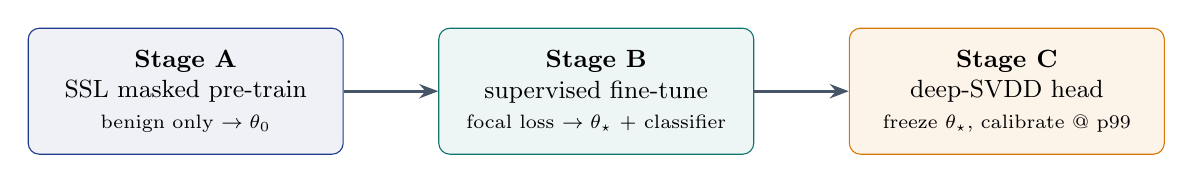
\begin{tikzpicture}[
  font=\small,
  stage/.style={draw=paneledge,rounded corners=4pt,minimum height=16mm,minimum width=40mm,align=center,inner sep=4pt},
  arr/.style={-{Stealth[length=2.4mm]},very thick,neutral}
]
\node[stage,fill=cool!7,draw=cool] (a) {\textbf{Stage A}\\SSL masked pre-train\\{\scriptsize benign only $\rightarrow \theta_0$}};
\node[stage,fill=accent!7,draw=accent,right=12mm of a] (b) {\textbf{Stage B}\\supervised fine-tune\\{\scriptsize focal loss $\rightarrow \theta_\star$ + classifier}};
\node[stage,fill=amber!9,draw=amber,right=12mm of b] (c) {\textbf{Stage C}\\deep-SVDD head\\{\scriptsize freeze $\theta_\star$, calibrate @ p99}};
\draw[arr] (a)--(b); \draw[arr] (b)--(c);
\end{tikzpicture}
\caption{Three-stage pipeline. Self-supervision learns ``normal'' once; the two
heads are trained cheaply on top of the frozen/fine-tuned encoder.}
\label{fig:pipe}
\end{figure}

\noindent Two operating modes share these same artifacts: a low-power
\emph{default} mode (smaller $K$, anomaly head only, target $<$2\,ms) and a
full-pipeline \emph{strong} mode ($K\!=\!32$, both heads, per-alert SHAP~\cite{shap}
attributions, target $<$10\,ms).

% =======================================================================
\section{Data and Feature Representation}

Flows are extracted from IoT-23~\cite{iot23} (Stratosphere Labs) packet captures with
\texttt{dpkt}; labels are joined from each Zeek \texttt{conn.log.labeled} by
5-tuple. Seven captures were used --- two from the initial prototype
(\texttt{34-1} Mirai, \texttt{8-1}) and five added for this report
(\texttt{1-1}, \texttt{3-1}, \texttt{20-1}, \texttt{21-1}, \texttt{42-1}) ---
chosen for attack-type diversity and manageable size. IoT-23 detailed labels map
onto the model's categories as: \texttt{PartOfAHorizontalPortScan}$\to$Recon,
\texttt{DDoS}$\to$DDoS, \texttt{Attack}$\to$BruteForce, and all
C\&C/Okiru/Torii$\to$Mirai. Per-class flows are \emph{water-filled} across source
captures (so each class draws from several scenarios) and balanced into a
31{,}960-flow training set (Fig.~\ref{fig:data}, left).

The single most consequential property of this data is \textbf{flow length}
(Fig.~\ref{fig:data}, right): benign connections and short scan/flood attacks are
tiny ($\sim$2--7 packets, median $\le$6), while brute-force flows are long
($\sim$30 packets). Over 99\% of the short-flow classes never reach the $K\!=\!32$
cap --- a fact that decides what any sequence model can and cannot separate.

\begin{figure}[H]
\centering
\begin{subfigure}{0.46\linewidth}
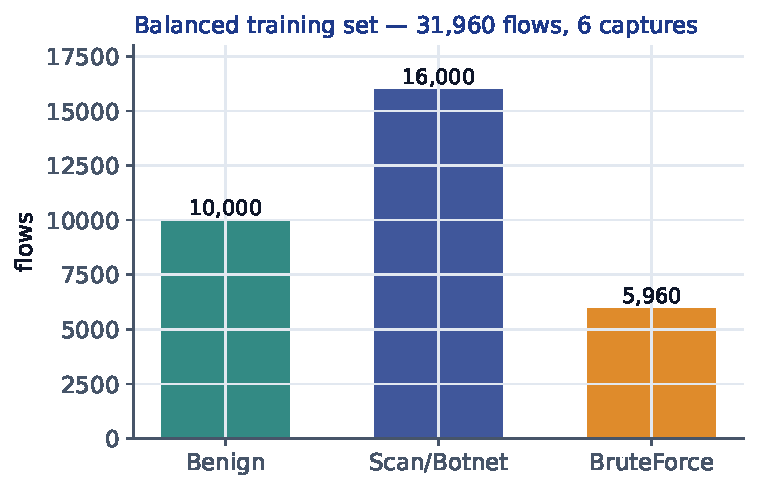
\includegraphics[width=\linewidth]{figs/fig_class_dist.pdf}
\caption{Balanced training set (3 classes).}
\end{subfigure}\hfill
\begin{subfigure}{0.52\linewidth}
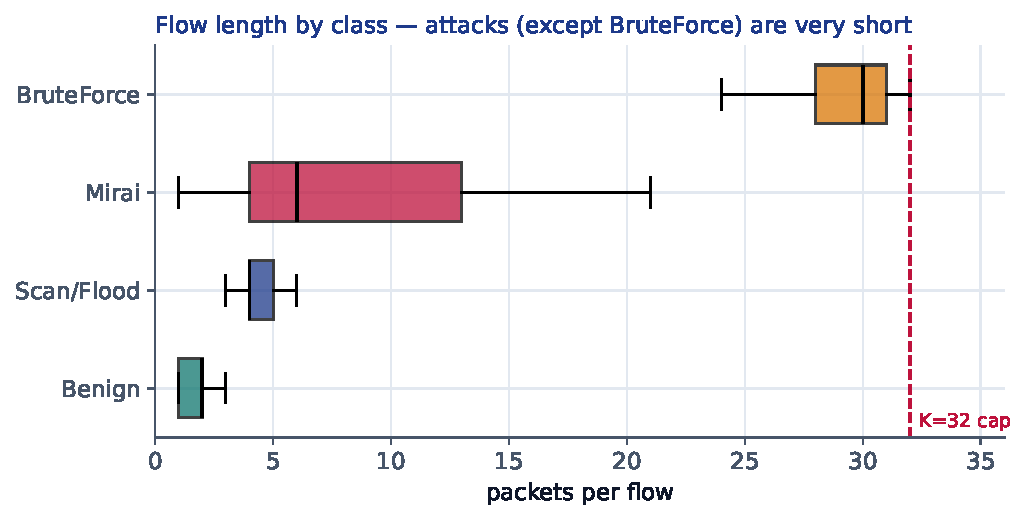
\includegraphics[width=\linewidth]{figs/fig_flow_length.pdf}
\caption{Flow length by class --- the decisive property.}
\end{subfigure}
\caption{Left: the class-balanced multi-capture dataset. Right: attacks (except
brute-force) are short connections; there is little sequence for a model to work with.}
\label{fig:data}
\end{figure}

\begin{figure}[H]
\centering
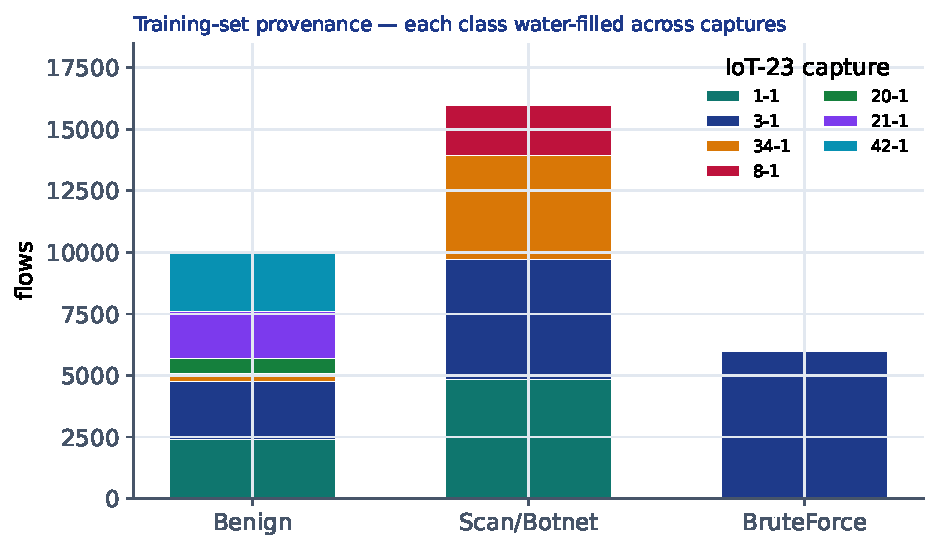
\includegraphics[width=0.64\linewidth]{figs/fig_provenance.pdf}
\caption{Each class is \emph{water-filled} across the seven captures so no single
scenario dominates --- Benign is drawn roughly evenly from six captures, which
broadens the notion of ``normal'' the anomaly head learns.}
\label{fig:prov}
\end{figure}

% =======================================================================
\section{Feature Significance and Preprocessing}

\subsection{Taming heavy-tailed features}
Raw traffic features --- packet sizes, byte counts, inter-arrival times --- are
heavy-tailed, spanning orders of magnitude; a single bulk transfer would dominate
any distance-based score. We compress the tail with a $\log(1{+}x)$ /
Yeo--Johnson~\cite{yeojohnson} power transform, then standardise
(Fig.~\ref{fig:logt}). The direction matters: $\log$ compacts the right tail,
$\exp$ would stretch it the wrong way.

\begin{figure}[H]
\centering
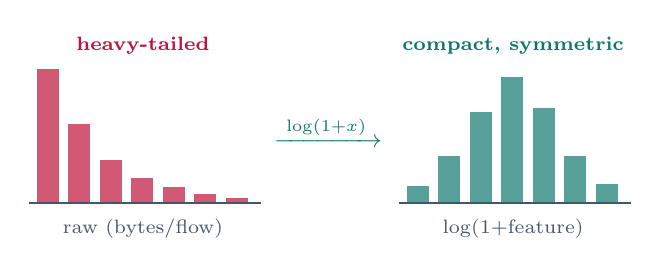
\begin{tikzpicture}[font=\small]
  \foreach \x/\h in {0/1.7,0.4/1.0,0.8/0.55,1.2/0.32,1.6/0.2,2.0/0.11,2.4/0.06}
     {\fill[rose!70] (\x,0) rectangle ++(0.28,\h);}
  \draw[neutral,thick] (-0.1,0)--(2.85,0);
  \node[rose,font=\bfseries\scriptsize] at (1.35,2.0) {heavy-tailed};
  \node[font=\scriptsize\color{neutral}] at (1.35,-0.32) {raw (bytes/flow)};
  \node[accent] at (3.7,0.9) {$\xrightarrow{\;\log(1{+}x)\;}$};
  \begin{scope}[shift={(4.7,0)}]
    \foreach \x/\h in {0/0.22,0.4/0.6,0.8/1.15,1.2/1.6,1.6/1.2,2.0/0.6,2.4/0.24}
       {\fill[accent!70] (\x,0) rectangle ++(0.28,\h);}
    \draw[neutral,thick] (-0.1,0)--(2.85,0);
    \node[accent,font=\bfseries\scriptsize] at (1.35,2.0) {compact, symmetric};
    \node[font=\scriptsize\color{neutral}] at (1.35,-0.32) {$\log(1{+}\text{feature})$};
  \end{scope}
\end{tikzpicture}
\caption{The log/Yeo--Johnson transform pulls the long right tail (rose) into a
compact, near-symmetric distribution (amber) so distances reflect the bulk of the
data, not a few outliers.}
\label{fig:logt}
\end{figure}

\subsection{Ranking, then confirming}
Feature \emph{significance} for the classical baselines is decided by mutual
information and SHAP~\cite{shap}; t-SNE~\cite{tsne} / UMAP~\cite{umap} only
\emph{confirm} separability --- they are visualisation tools, not rankers (their
axes are nonlinear blends of all inputs). For the Mamba arm there is no
hand-picked vector: the encoder learns its own embedding $z$, and the right check
is a t-SNE of $z$ (Fig.~\ref{fig:tsne}).

\begin{figure}[H]
\centering
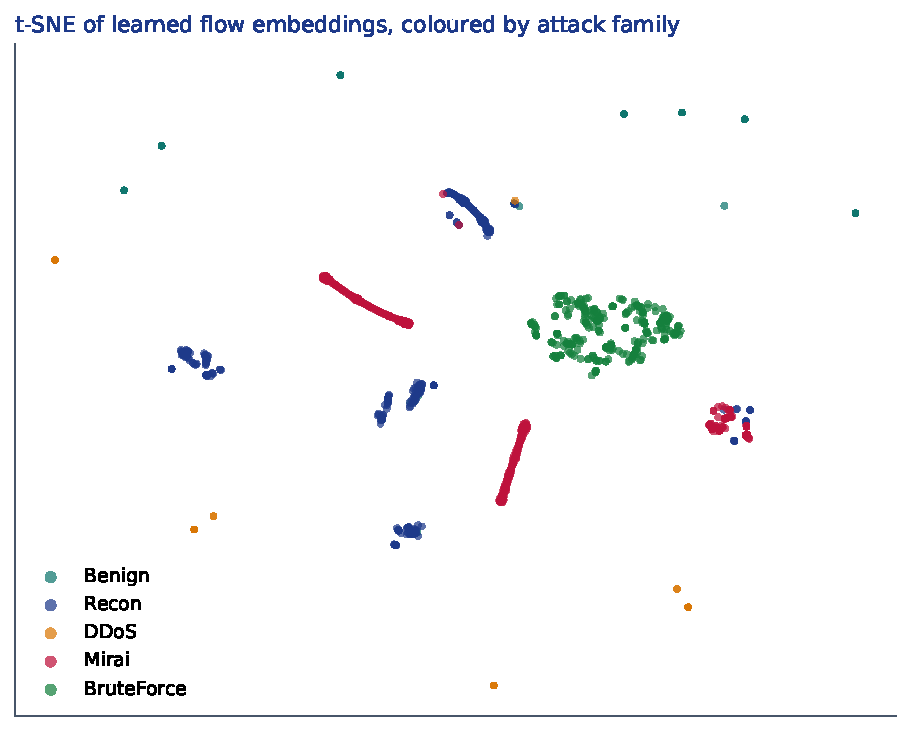
\includegraphics[width=0.66\linewidth]{figs/fig_tsne.pdf}
\caption{t-SNE of the learned flow embeddings (1{,}411 flows). \textbf{BruteForce}
(long, $\sim$30-packet) and \textbf{Mirai} form distinct clusters; \textbf{Recon}
fragments into several small clusters; \textbf{DDoS} (only 211 flows) is too sparse
to place. A caution: t-SNE's 2-D proximity is \emph{not} classifier separability
--- a capture-controlled pairwise test (Table~\ref{tab:pairwise}) shows Mirai is
\emph{fully} separable from the scan classes, while Recon$\leftrightarrow$DDoS is
the genuinely fused pair.}
\label{fig:tsne}
\end{figure}

\subsection{The anomaly sphere}
The zero-day head is a deep-SVDD~\cite{deepsvdd} one-class scorer: a learned
projection $\mathbb{R}^{128}\!\to\!\mathbb{R}^{32}$ packs benign embeddings into a
minimum-volume ball around a centre $c$; a flow beyond radius $R$ (99th benign
percentile, 1\% FPR) is flagged (Fig.~\ref{fig:sphere}). An L2-normalised
angular-cap variant is a clean A/B alternative. In practice the benign scores pack
tightly near the centre while attacks spread out (Fig.~\ref{fig:anomdist}).

\begin{figure}[H]
\centering
\begin{minipage}[c]{0.34\linewidth}
\centering
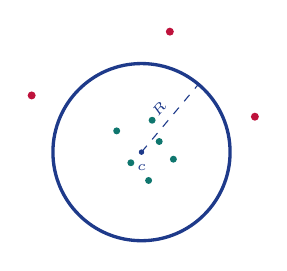
\begin{tikzpicture}[font=\small,scale=0.9]
  \draw[cool,very thick] (0,0) circle (1.25);
  \draw[cool,dashed] (0,0)--(50:1.25) node[midway,above,sloped,font=\tiny\color{cool}]{$R$};
  \fill[cool] (0,0) circle (1.1pt) node[below=1pt,font=\tiny\color{cool}]{$c$};
  \foreach \p in {(0.25,0.15),(-0.35,0.3),(0.1,-0.4),(-0.15,-0.15),(0.45,-0.1),(0.15,0.45)}
     {\fill[accent] \p circle (1.4pt);}
  \foreach \p in {(1.6,0.5),(-1.55,0.8),(0.4,1.7)} {\fill[rose] \p circle (1.6pt);}
\end{tikzpicture}\\[2pt]
{\scriptsize deep-SVDD ball}
\end{minipage}\hfill
\begin{minipage}[c]{0.62\linewidth}
\centering
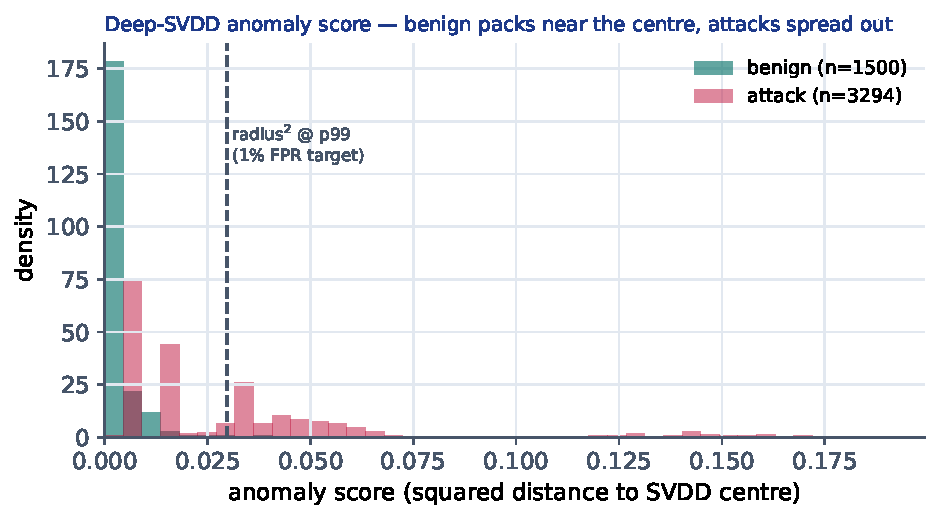
\includegraphics[width=\linewidth]{figs/fig_anomdist.pdf}
\end{minipage}
\caption{Left: deep-SVDD packs benign embeddings (amber) into a ball of radius $R$
around $c$; anomalies (rose) fall outside. Right: the measured score distribution
--- benign concentrates near zero, attacks spread past the calibrated radius.}
\label{fig:sphere}
\label{fig:anomdist}
\end{figure}

% =======================================================================
\section{Experimental Journey}

The project evolved through a sequence of experiments, each of which produced a
concrete finding rather than just a number (Table~\ref{tab:journey},
Fig.~\ref{fig:evo}).

\begin{table}[H]
\centering\small
\caption{The experimental journey. Macro-F1 is over the classes present in each setup.}
\label{tab:journey}
\renewcommand{\arraystretch}{1.15}
\begin{tabularx}{\linewidth}{@{}p{0.28\linewidth}cccX@{}}
\toprule
\textbf{Experiment} & \textbf{Acc} & \textbf{Macro-F1} & \textbf{Anom.} & \textbf{Finding} \\
\midrule
34-1, 4-class (random split)      & 0.963 & 0.793 & 0.994 & Anomaly head excellent; DDoS$\leftrightarrow$Recon confused \\
34-1 + stratify + focal           & --    & 0.77 / 0.67 & 0.99 & Reweighting \emph{see-saws} $\Rightarrow$ genuine overlap \\
34-1 merged, 3-class              & 0.991 & \textbf{0.957} & 0.994 & Merging DDoS+Recon $\to$ Scan/Flood fixes it \\
34-1{+}8-1 combined, 4-class      & --    & 0.686 & 0.991 & Pure-Mirai capture \emph{regressed} the classifier \\
Multi-source, 4-class             & 0.906 & 0.895 & 0.913 & New BruteForce class (F1 0.996); Mirai recall 0.60 \\
Multi-source, Mirai$\uparrow$2.5$\times$ & 0.830 & 0.832 & --   & See-saw again $\Rightarrow$ Mirai/Scan overlap \\
\textbf{Multi-source, 3-class (final)} & \textbf{0.982} & \textbf{0.984} & \textbf{0.935} & Align taxonomy with separability \\
\bottomrule
\end{tabularx}
\end{table}

\begin{figure}[H]
\centering
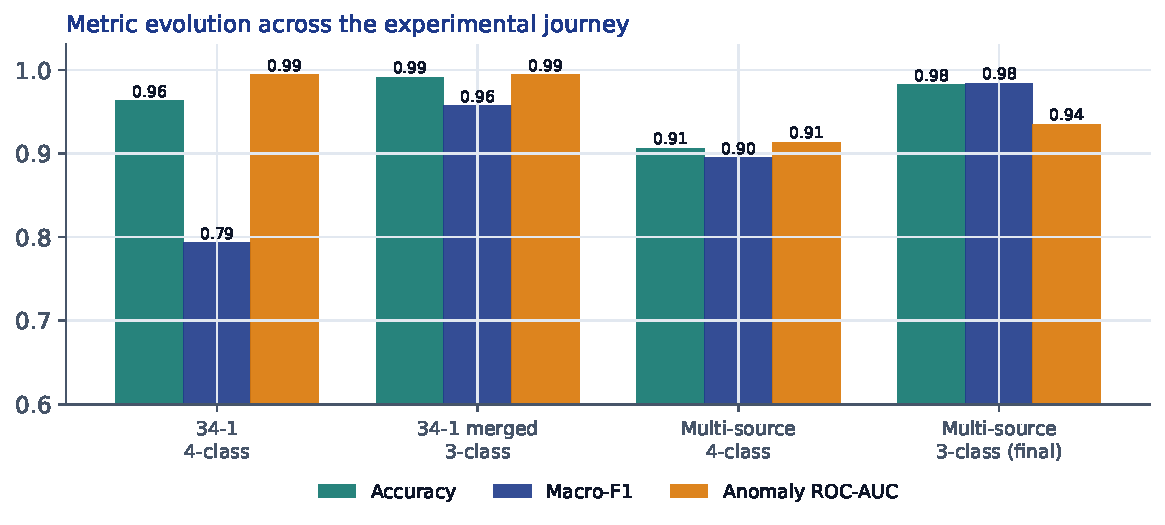
\includegraphics[width=0.82\linewidth]{figs/fig_metric_evolution.pdf}
\caption{Metric evolution across the four milestone models. Numbers span evolving
class sets and test splits, so they read as a trajectory rather than a strict
apples-to-apples comparison.}
\label{fig:evo}
\end{figure}

\subsection{From one capture to many}
The prototype on a single Mirai capture (\texttt{34-1}) already validated the
central bet --- the benign-trained anomaly head hit \textbf{ROC-AUC 0.994} on
real malware, at sub-6\,ms latency. But the supervised classifier persistently
confused DDoS with Recon. Two attempted fixes (stratified splits, per-class focal
weights) only made the errors \emph{swap direction}: upweighting one class
sacrificed the other. This \emph{see-saw} is the signature of genuine feature
overlap, not class imbalance. Merging the two indistinguishable classes into a
single \textbf{Scan/Flood} class resolved it cleanly (macro-F1 0.957).

Scaling to more captures added a genuinely new, well-separated class ---
\textbf{BruteForce} (F1 0.996) --- and a much more diverse benign set, at the
cost of a lower but \emph{more honest} anomaly ROC-AUC (0.913 vs.\ the inflated
single-capture 0.994). It also surfaced the same pathology one level up: the
now-separate \textbf{Mirai} class was confused with Scan/Flood (recall 0.60).

\subsection{The see-saw, and why longer sequences cannot help}
Upweighting Mirai $2.5\times$ drove its recall to 0.999 --- but collapsed
Scan/Flood recall to 0.503 and dropped overall accuracy to 0.830
(Fig.~\ref{fig:seesaw}). The confusion did not vanish; it flipped and grew. The
obvious next idea --- longer sequences ($K\!=\!64$) to let persistent C\&C diverge
from short scans --- was ruled out for \emph{free} by the length analysis: over
99\% of these flows never reach even 32 packets, so there are no extra packets to
use. Mirai botnet traffic \emph{is} partly horizontal port-scanning; over the
first $\sim$6 packets it is genuinely indistinguishable from the scan class.

\begin{figure}[H]
\centering
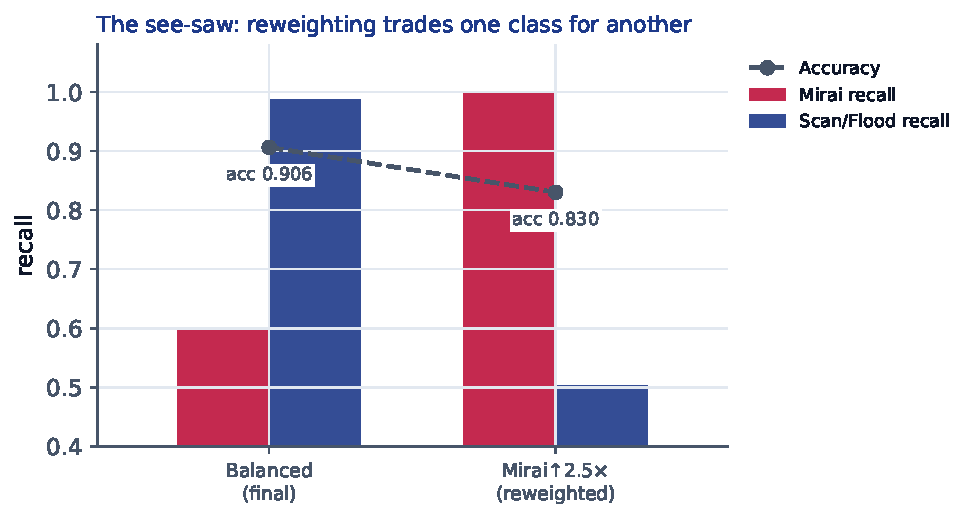
\includegraphics[width=0.5\linewidth]{figs/fig_seesaw.pdf}
\caption{Reweighting is a zero-sum trade between two overlapping classes:
Mirai recall rises only as Scan/Flood recall falls, and accuracy drops.}
\label{fig:seesaw}
\end{figure}

% =======================================================================
\section{Final Model and Results}

Aligning the taxonomy with what the features can resolve --- Benign, a combined
\textbf{Scan/Botnet} class (DDoS, Recon and Mirai, all short-flow attacks), and
\textbf{BruteForce} --- gives a clean, high-accuracy detector. Trained for
3 stages $\times$ 6 epochs on 31{,}960 flows with a stratified split and mild
$\sqrt{}$-frequency focal weights, it reaches \textbf{98.2\,\% accuracy}
(Table~\ref{tab:final}, Fig.~\ref{fig:cm}).

\begin{table}[H]
\centering\small
\caption{Final three-class model on the held-out test set (4{,}794 flows).}
\label{tab:final}
\renewcommand{\arraystretch}{1.15}
\begin{tabular}{@{}lrrrr@{}}
\toprule
\textbf{Class} & \textbf{Precision} & \textbf{Recall} & \textbf{F1} & \textbf{N} \\
\midrule
Benign      & 0.989 & 0.955 & 0.972 & 1500 \\
Scan/Botnet & 0.974 & 0.993 & 0.983 & 2400 \\
BruteForce  & 0.994 & 0.999 & \textbf{0.997} & 894 \\
\midrule
Macro avg    & 0.986 & 0.982 & \textbf{0.984} & 4794 \\
Weighted avg & 0.982 & 0.982 & 0.982 & 4794 \\
\bottomrule
\end{tabular}
\quad
\renewcommand{\arraystretch}{1.15}
\begin{tabular}{@{}lr@{}}
\toprule
\textbf{Metric} & \textbf{Value} \\
\midrule
Accuracy         & \textbf{98.2\%} \\
Anomaly ROC-AUC  & \textbf{0.935} \\
Anomaly PR-AUC   & 0.959 \\
Latency p50/p95  & 5.0 / 6.5\,ms \\
Model size       & 2.0\,MB \\
\bottomrule
\end{tabular}
\end{table}

\begin{figure}[H]
\centering
\begin{subfigure}{0.62\linewidth}
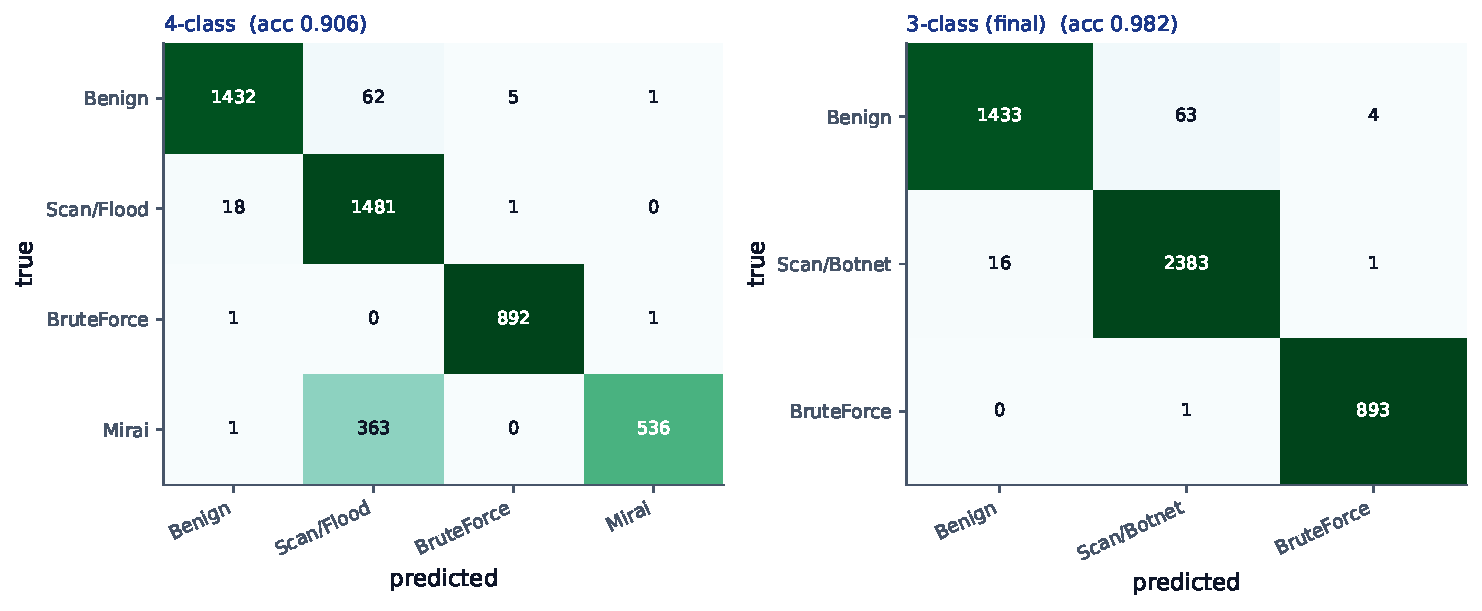
\includegraphics[width=\linewidth]{figs/fig_confusion.pdf}
\caption{Row-normalised confusion: 4-class (left) vs.\ final 3-class (right).}
\end{subfigure}\hfill
\begin{subfigure}{0.35\linewidth}
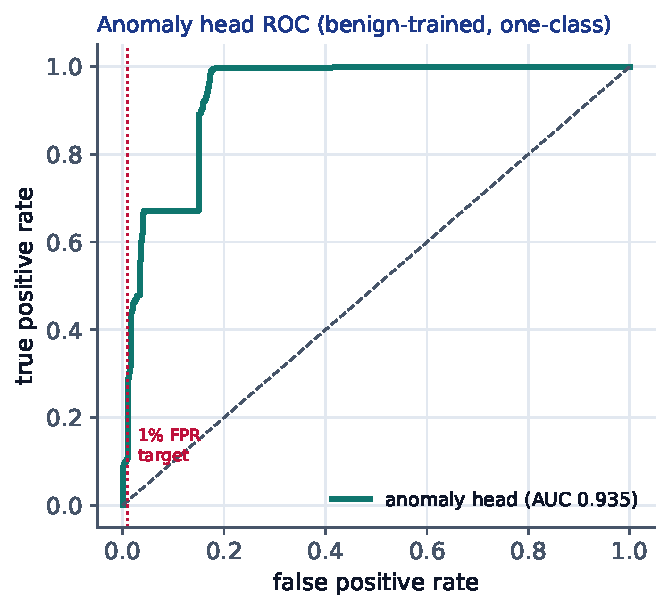
\includegraphics[width=\linewidth]{figs/fig_roc.pdf}
\caption{Anomaly-head ROC.}
\end{subfigure}
\caption{Left: merging the inseparable short-flow attacks turns the 4-class
Mirai$\to$Scan smear into a near-diagonal 3-class matrix. Right: the one-class
anomaly head at ROC-AUC 0.935 on hard, multi-source data.}
\label{fig:cm}
\end{figure}

\begin{figure}[H]
\centering
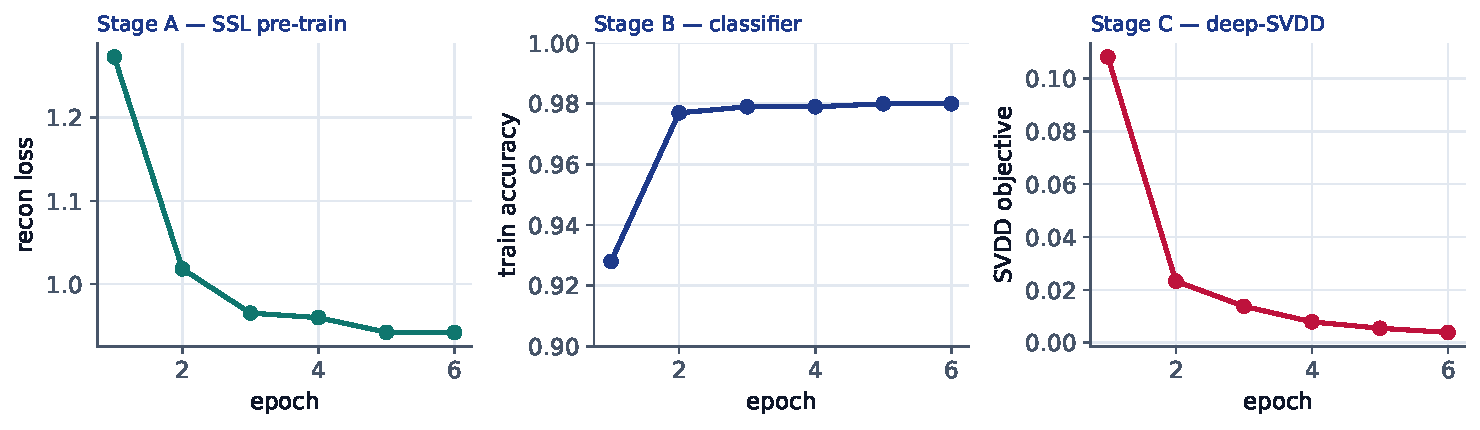
\includegraphics[width=0.92\linewidth]{figs/fig_training_curves.pdf}
\caption{Training convergence (final 3-class run). All three stages plateau well
inside 6 epochs; the accuracy ceiling is data/feature-bound, not
under-training.}
\label{fig:curves}
\end{figure}

% =======================================================================
\section{Deployment and Quantization}

The detector must fit on Raspberry-Pi-class hardware, so the deployed model is
\emph{quantised} --- weights and activations stored in fewer bits than fp32. The
wrinkle is that most quantisation work targets transformers, whereas Mamba's
\emph{selective state-space core} carries activation outliers that compound
through its recurrence and resist naive int8.

\keybox{Strategy.}{\emph{Mixed precision} --- int8 for the linear projections
(which dominate the parameter count and quantise cleanly), fp16 for the
outlier-sensitive selective-scan core (Fig.~\ref{fig:quant}). Most of the size
saving comes from the projections anyway; quantisation-aware training is the
fallback if fp16 still costs accuracy on the SSM core~\cite{qmamba,mambaquant,ptq4ssm}.}

\begin{figure}[H]
\centering
\resizebox{0.92\linewidth}{!}{%
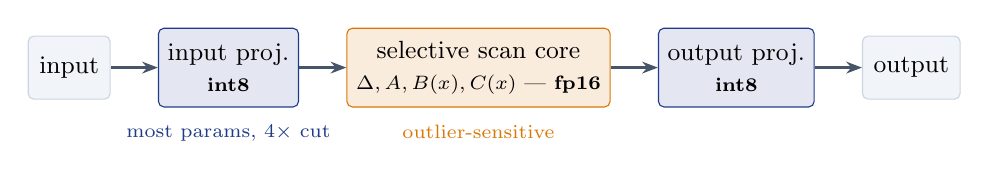
\begin{tikzpicture}[
  font=\small,
  d/.style={draw=paneledge,fill=panel,rounded corners=2pt,minimum height=8mm,inner sep=4pt,align=center},
  i8/.style={draw=cool,fill=cool!12,rounded corners=2pt,minimum height=10mm,align=center},
  f16/.style={draw=amber,fill=amber!14,rounded corners=2pt,minimum height=10mm,align=center},
  a/.style={-{Stealth[length=2mm]},thick,neutral}
]
\node[d] (in) {input};
\node[i8,right=6mm of in] (p1) {input proj.\\{\scriptsize\textbf{int8}}};
\node[f16,right=6mm of p1] (ssm) {selective scan core\\{\scriptsize $\Delta,A,B(x),C(x)$ --- \textbf{fp16}}};
\node[i8,right=6mm of ssm] (p2) {output proj.\\{\scriptsize\textbf{int8}}};
\node[d,right=6mm of p2] (out) {output};
\draw[a] (in)--(p1); \draw[a] (p1)--(ssm); \draw[a] (ssm)--(p2); \draw[a] (p2)--(out);
\node[cool,below=1mm of p1,font=\scriptsize] {most params, $4\times$ cut};
\node[amber,below=1mm of ssm,font=\scriptsize] {outlier-sensitive};
\end{tikzpicture}}
\caption{Mixed-precision split inside a Mamba block: int8 projections (which hold
most weights), fp16 selective-scan core --- the compromise across the 2024--25
Mamba quantisation literature (Q-Mamba, MambaQuant, PTQ4SSM).}
\label{fig:quant}
\end{figure}

The plan reports three precisions so the operator can trade size against accuracy
(Table~\ref{tab:quant}). \textbf{These are design projections, not measured} ---
the shipped \texttt{detector.pt} is the 2\,MB fp32 model, and the int8 conversion
plus the on-device (Raspberry-Pi) benchmark remain outstanding (\S9).

\begin{table}[H]
\centering\small
\caption{Planned quantisation configurations (projected, per the deployment design).}
\label{tab:quant}
\renewcommand{\arraystretch}{1.15}
\begin{tabularx}{0.82\linewidth}{@{}Xccc@{}}
\toprule
\textbf{Configuration} & \textbf{Size} & \textbf{p95 latency} & \textbf{Accuracy hit} \\
\midrule
fp32 (baseline)                        & $1.0\times$          & $1.0\times$        & --- \\
int8 PTQ everywhere                    & $0.25\times$         & ${\sim}0.5\times$  & risk on SSM core \\
\textbf{Mixed precision (recommended)} & $\approx 0.30\times$ & ${\sim}0.55\times$ & smallest drop \\
\bottomrule
\end{tabularx}
\end{table}

% =======================================================================
\section{Continual and Progressive Learning}

Attack landscapes drift, so a deployed detector must absorb new attack variants
without forgetting old ones. The hard case is \emph{correlation}: a new DDoS
variant that resembles standard DDoS. Three failure modes lurk --- catastrophic
forgetting, probability-mass theft (a new class stealing confidence from old
ones), and spurious hard labels on ambiguous flows. The update protocol
(Fig.~\ref{fig:continual}) keeps the expensive encoder \emph{frozen} and touches
only the cheap heads, with four defences in order: (1) a replay buffer of
$\sim$100--500 flows per existing class; (2) knowledge distillation
(learning-without-forgetting) against the previous head; (3) an embedding-space
check that decides \emph{add} (tight and far $\rightarrow$ new class),
\emph{merge} (overlapping $\rightarrow$ sub-class), or \emph{separate} (scattered
$\rightarrow$ margin fine-tune); and (4) an automatic rollback if any existing
class's F1 regresses beyond an agreed threshold.

\begin{figure}[H]
\centering
\resizebox{\linewidth}{!}{%
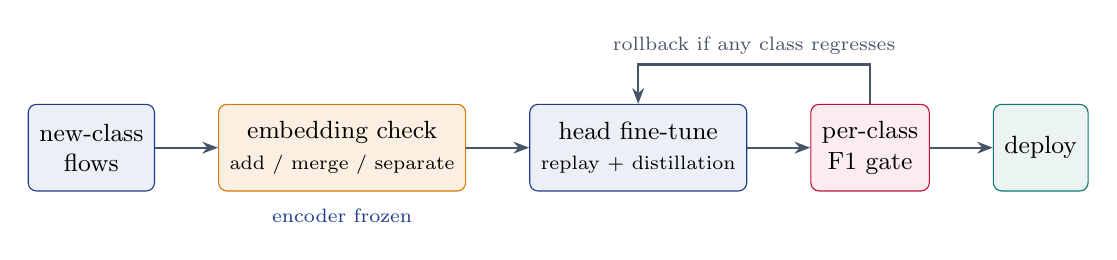
\begin{tikzpicture}[
  font=\small,
  b/.style={draw=cool,fill=cool!8,rounded corners=3pt,minimum height=11mm,align=center,inner sep=4pt},
  dec/.style={draw=amber,fill=amber!12,rounded corners=3pt,minimum height=11mm,align=center,inner sep=4pt},
  g/.style={draw=rose,fill=rose!8,rounded corners=3pt,minimum height=11mm,align=center,inner sep=4pt},
  a/.style={-{Stealth[length=2mm]},thick,neutral}
]
\node[b] (new) {new-class\\flows};
\node[dec,right=8mm of new] (emb) {embedding check\\{\scriptsize add / merge / separate}};
\node[b,right=8mm of emb] (ft) {head fine-tune\\{\scriptsize replay + distillation}};
\node[g,right=8mm of ft] (gate) {per-class\\F1 gate};
\node[b,right=8mm of gate,fill=accent!8,draw=accent] (dep) {deploy};
\draw[a] (new)--(emb); \draw[a] (emb)--(ft); \draw[a] (ft)--(gate); \draw[a] (gate)--(dep);
\draw[a] (gate.north) -- ++(0,5mm) -| (ft.north)
   node[pos=0.25,above,font=\scriptsize\color{rose}] {rollback if any class regresses};
\node[cool,below=1mm of emb,font=\scriptsize] {encoder frozen};
\end{tikzpicture}}
\caption{The progressive-learning update: only the cheap heads change; a replay +
distillation fine-tune is gated by a per-class F1 check, with automatic rollback.}
\label{fig:continual}
\end{figure}

% =======================================================================
\section{Analysis: what the features can and cannot resolve}

The governing result of the whole journey is a single structural fact:

\keybox{Design finding.}{Payload-free features on short flows separate traffic by
\emph{flow structure} (benign $\sim$3 pkts, short scan/botnet $\sim$5 pkts, long
brute-force $\sim$30 pkts) more than by fine attack family. A capture-controlled
pairwise test is precise (Table~\ref{tab:pairwise}): \textbf{Mirai is fully
separable} from the scan classes, but \textbf{Recon$\leftrightarrow$DDoS is
near-chance} --- both are short horizontal-scan/flood patterns overlapping in the
first $\sim$6 packets. So the genuinely inseparable pair is Recon/DDoS; Mirai is
merged in the \emph{flat} 3-class model only for robustness against cross-capture
variety, and the hierarchical CNN layer (\S\ref{sec:cnn}) recovers it.}

\begin{table}[H]
\centering\small
\caption{Pairwise separability within a single capture (34-1), so the score
reflects attack behaviour, not capture identity. Random-forest 5-fold accuracy.}
\label{tab:pairwise}
\renewcommand{\arraystretch}{1.15}
\begin{tabular}{@{}lcc@{}}
\toprule
\textbf{Pair} & \textbf{5-fold accuracy} & \textbf{Verdict} \\
\midrule
Recon vs DDoS  & 0.736 & near-chance --- \emph{fused} \\
Recon vs Mirai & \textbf{1.000} & fully separable \\
DDoS vs Mirai  & \textbf{1.000} & fully separable \\
\bottomrule
\end{tabular}
\end{table}

This is not a failure of the model but an honest measurement of the information
content of the representation. It has two direct consequences: (i) the
\textbf{three-class taxonomy} is the right granularity for these features, and
(ii) recovering the finer attack families would require information the current
input lacks --- \emph{flow-level metadata} (duration, byte counts, destination-port
diversity, connection state), not more packets. The anomaly head --- the
project's zero-day centrepiece --- is unaffected by this classifier question and
remains strong (ROC-AUC 0.935) on diverse, realistic traffic; its earlier 0.994
was inflated by a single Mirai-dominated capture. \emph{Tooling:} heavy-tailed
features are Yeo--Johnson~\cite{yeojohnson} transformed before standardisation;
embedding separability is verified with t-SNE~\cite{tsne} / UMAP~\cite{umap}; and a
per-window device-communication graph branch (E-GraphSAGE~\cite{egraphsage}) is a
planned extension.

% =======================================================================
\section{A CNN Fine-Layer: Sub-Classifying Scan/Botnet}
\label{sec:cnn}

The Scan/Botnet class deliberately fuses three attack families (DDoS, Recon,
Mirai). A natural --- and suggested --- extension is to leave the detector intact
and add a \emph{CNN as a dedicated second-stage layer} whose only job is to split
that class back into its families (Fig.~\ref{fig:hierarch}). We evaluate this two
ways.

\begin{figure}[H]
\centering
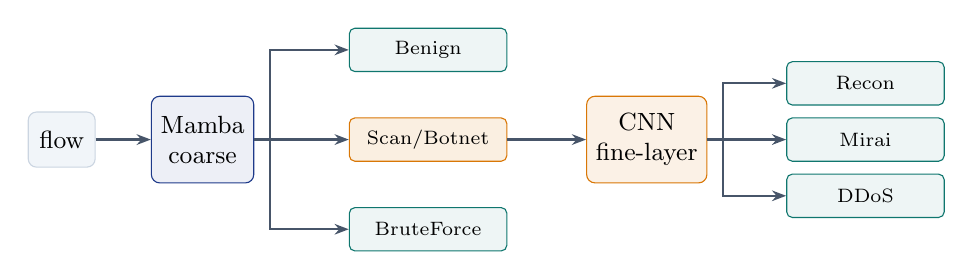
\begin{tikzpicture}[
  font=\small,
  box/.style={draw=paneledge,fill=panel,rounded corners=3pt,minimum height=7mm,inner sep=4pt,align=center},
  enc/.style={draw=cool,fill=cool!8,rounded corners=3pt,minimum height=11mm,align=center},
  cnn/.style={draw=amber,fill=amber!10,rounded corners=3pt,minimum height=11mm,align=center},
  leaf/.style={draw=accent,fill=accent!7,rounded corners=2pt,minimum height=5.5mm,minimum width=20mm,inner sep=2pt,align=center,font=\scriptsize},
  arr/.style={-{Stealth[length=1.8mm]},thick,neutral}
]
\node[box] (in) {flow};
\node[enc,right=7mm of in] (co) {Mamba\\coarse};
\node[leaf,above right=3mm and 12mm of co] (be) {Benign};
\node[leaf,right=12mm of co,fill=amber!12,draw=amber] (sb) {Scan/Botnet};
\node[leaf,below right=3mm and 12mm of co] (bf) {BruteForce};
\node[cnn,right=10mm of sb] (cn) {CNN\\fine-layer};
\node[leaf,right=10mm of cn] (mi) {Mirai};
\node[leaf,above=1.5mm of mi] (re) {Recon};
\node[leaf,below=1.5mm of mi] (dd) {DDoS};
\draw[arr] (in)--(co);
\draw[arr] (co.east)-- ++(2mm,0) |- (be.west);
\draw[arr] (co.east) -- (sb.west);
\draw[arr] (co.east)-- ++(2mm,0) |- (bf.west);
\draw[arr] (sb)--(cn);
\draw[arr] (cn.east)-- ++(2mm,0) |- (re.west);
\draw[arr] (cn.east)-- (mi.west);
\draw[arr] (cn.east)-- ++(2mm,0) |- (dd.west);
\end{tikzpicture}
\caption{Hierarchical design. The robust coarse detector routes each flow; a CNN
fine-layer, trained only on Scan/Botnet flows, names the attack family.}
\label{fig:hierarch}
\end{figure}

\subsection{Does the architecture matter? CNN vs.\ Mamba vs.\ XGBoost}
Training a CNN, our Mamba encoder, and an order-agnostic XGBoost on the identical
three-way task (Recon/DDoS/Mirai) gives a clear verdict (Fig.~\ref{fig:cnncmp}):
\begin{itemize}[leftmargin=1.4em,itemsep=1pt,topsep=2pt]
  \item The \textbf{CNN matches but does not beat the Mamba} --- on both settings
  they converge to identical predictions (differing only in confidence). The
  useful idea is the \emph{hierarchy}, not the architecture.
  \item Both sequence models \textbf{beat order-agnostic XGBoost} (0.75 vs.\ 0.60,
  single-capture), so keeping packet order helps the fine split too.
  \item XGBoost's \emph{perfect} 1.00 on multi-capture data was the tell for
  \textbf{capture leakage}: because each family is sourced from different captures,
  a model can fingerprint the \emph{capture} (via TTL, window size) instead of the
  attack. The capture-controlled numbers ($\sim$0.75) are the honest ones.
\end{itemize}

\begin{figure}[H]
\centering
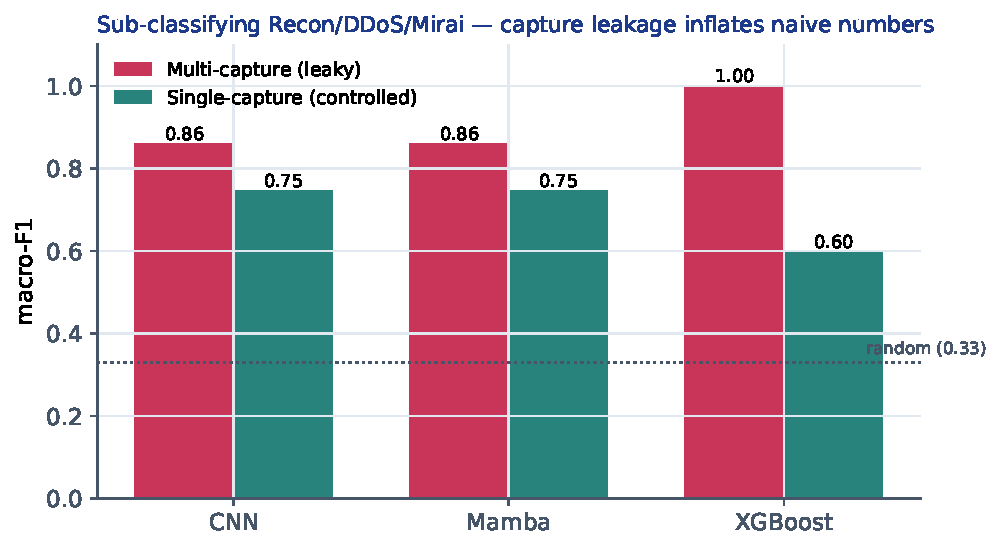
\includegraphics[width=0.66\linewidth]{figs/fig_cnn_compare.pdf}
\caption{Fine-split macro-F1. All three models drop sharply from multi-capture to
single-capture --- especially XGBoost (1.00$\to$0.60) --- exposing how much of the
naive score was capture identity, not attack behaviour.}
\label{fig:cnncmp}
\end{figure}

\subsection{The end-to-end hierarchical detector}
Wiring the CNN fine-layer beneath the coarse Mamba upgrades the three-class
detector into a five-class one that \emph{names} the attack family
(Table~\ref{tab:hier}, Fig.~\ref{fig:hiercm}). It reaches \textbf{91.8\,\%
accuracy} and cleanly recovers DDoS, Mirai and BruteForce; Recon is the weak point
(some flows read as Mirai). The flat coarse model alone scores 0.985 on the 3-way
but cannot name families --- the fine-layer is what buys that capability.

\begin{figure}[H]
\centering
\begin{subfigure}{0.44\linewidth}
\centering\small
\renewcommand{\arraystretch}{1.15}
\begin{tabular}{@{}lrrr@{}}
\toprule
\textbf{Class} & \textbf{P} & \textbf{R} & \textbf{F1} \\
\midrule
Benign      & 0.977 & 0.960 & 0.969 \\
Recon       & 0.946 & 0.698 & 0.803 \\
DDoS        & 1.000 & 1.000 & 1.000 \\
Mirai       & 0.781 & 1.000 & 0.877 \\
BruteForce  & 1.000 & 1.000 & 1.000 \\
\midrule
\multicolumn{4}{@{}l}{Accuracy \textbf{0.918} \; Macro-F1 \textbf{0.930}} \\
\bottomrule
\end{tabular}
\captionsetup{skip=2pt}\caption{Per-class (5-way).}
\label{tab:hier}
\end{subfigure}\hfill
\begin{subfigure}{0.52\linewidth}
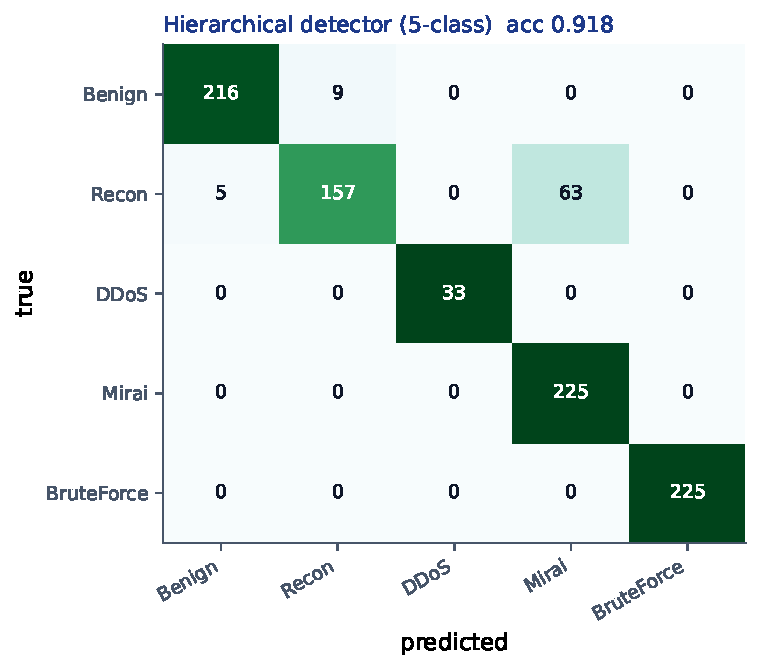
\includegraphics[width=\linewidth]{figs/fig_hier_confusion.pdf}
\caption{End-to-end confusion.}
\end{subfigure}
\caption{The hierarchical detector names four attack states plus benign at
91.8\,\% accuracy; the residual is Recon read as Mirai.}
\label{fig:hiercm}
\end{figure}

\keybox{Honesty caveat.}{These multi-capture fine numbers are inflated by capture
leakage: DDoS's perfect score reflects its unique source capture, and the
confusion pattern \emph{shifts} with capture composition (single-capture
DDoS$\to$Recon; multi-capture Recon$\to$Mirai) --- the fingerprint of confounding.
The trustworthy fine-split ceiling is $\sim$0.75 macro-F1, with
DDoS$\leftrightarrow$Recon the genuine limit. A leave-one-capture-out evaluation
is the deployment-honest next step.}

% =======================================================================
\section{Evaluation Design}

Beyond the results reported above, the full evaluation plan pits the detector
against four baselines, each isolating a different question
(Table~\ref{tab:base}), plus two stress tests: \textbf{FGSM} adversarial
perturbations clipped to valid packet ranges~\cite{advids}, and a
\textbf{leave-one-class-out} zero-day proxy --- hide an attack class during
supervised training, then measure how well the benign-trained anomaly head still
flags it. Headline metrics are per-class P/R/F1, PR-AUC (the honest metric under
imbalance), latency p50/p95/p99, and int8 model size.

\begin{table}[H]
\centering\small
\caption{The four baselines, and the question each isolates.}
\label{tab:base}
\renewcommand{\arraystretch}{1.2}
\begin{tabularx}{\linewidth}{@{}lX@{}}
\toprule
\textbf{Baseline} & \textbf{Role} \\
\midrule
ET-BERT~\cite{etbert}          & published-SOTA \emph{upper bound} (accuracy ceiling) \\
CNN-BiLSTM on aggregates       & \emph{representation control} --- does keeping packet order help? \\
XGBoost on aggregates          & classical \emph{accuracy floor} \\
Isolation Forest               & unsupervised \emph{anomaly floor} for the zero-day head \\
\bottomrule
\end{tabularx}
\end{table}

The deep detector earns its complexity only if it beats the classical floor on
zero-day detection, cross-dataset transfer, and adversarial robustness; where
XGBoost matches in-distribution, that is reported as an honest finding.

% =======================================================================
\section{Project Timeline}

The eight-week internship (DOJ 11\textsuperscript{th} May 2026) progressed from
data plumbing to a validated multi-source detector (Fig.~\ref{fig:timeline}).

\begin{figure}[H]
\centering
\resizebox{0.9\linewidth}{!}{%
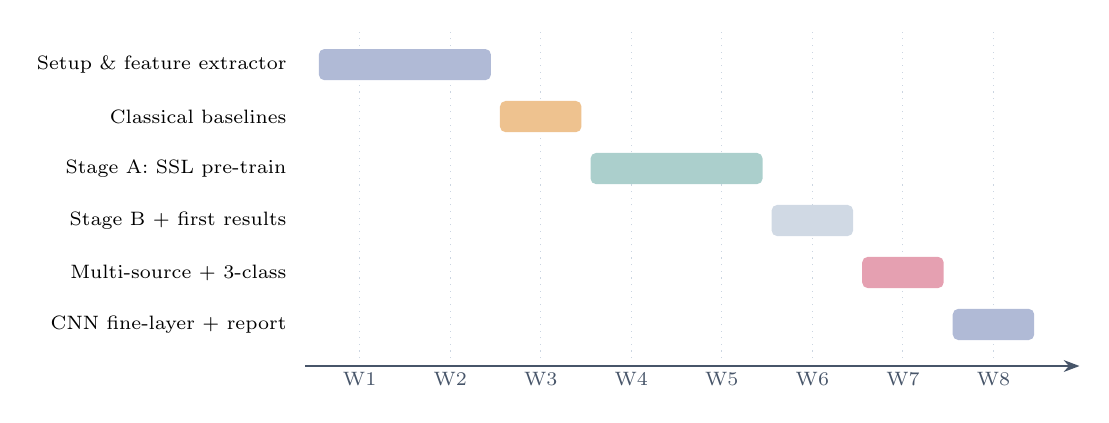
\begin{tikzpicture}[font=\scriptsize, x=1.15cm, y=0.66cm]
\foreach \w in {1,...,8}{
  \draw[paneledge,dotted] (\w,0.35)--(\w,6.7);
  \node[font=\scriptsize\color{neutral}] at (\w,-0.05){W\w};
}
\draw[neutral,thick,-{Stealth[length=2mm]}] (0.4,0.2)--(8.95,0.2);
\fill[cool!35,rounded corners=2pt]      (0.55,5.7) rectangle (2.45,6.3);
\node[anchor=east,font=\scriptsize] at (0.3,6){Setup \& feature extractor};
\fill[amber!45,rounded corners=2pt]     (2.55,4.7) rectangle (3.45,5.3);
\node[anchor=east,font=\scriptsize] at (0.3,5){Classical baselines};
\fill[accent!35,rounded corners=2pt]    (3.55,3.7) rectangle (5.45,4.3);
\node[anchor=east,font=\scriptsize] at (0.3,4){Stage A: SSL pre-train};
\fill[paneledge!90,rounded corners=2pt] (5.55,2.7) rectangle (6.45,3.3);
\node[anchor=east,font=\scriptsize] at (0.3,3){Stage B + first results};
\fill[rose!40,rounded corners=2pt]      (6.55,1.7) rectangle (7.45,2.3);
\node[anchor=east,font=\scriptsize] at (0.3,2){Multi-source + 3-class};
\fill[cool!35,rounded corners=2pt]      (7.55,0.7) rectangle (8.45,1.3);
\node[anchor=east,font=\scriptsize] at (0.3,1){CNN fine-layer + report};
\end{tikzpicture}}
\caption{Eight-week timeline: setup and extraction (W1--2), classical baselines
(W3), self-supervised pre-training (W4--5), supervised fine-tune and first
single-capture results (W6), multi-source data with the 3-class taxonomy (W7), and
the hierarchical CNN layer plus this report (W8).}
\label{fig:timeline}
\end{figure}

% =======================================================================
\section{Limitations and Next Steps}

\begin{itemize}[leftmargin=1.4em,itemsep=2pt,topsep=2pt]
\item \hd{Leave-one-capture-out evaluation.} The CNN fine-layer (previous section)
is built and works end-to-end (91.8\,\%), but its fine-split scores benefit from
capture leakage; a leave-one-capture-out protocol is the deployment-honest way to
report generalisation.
\item \hd{Flow-level features} are the principled lever for finer attack-family
resolution --- and would likely help the residual benign$\leftrightarrow$scan
boundary too.
\item \hd{Broader evaluation}, per the proposal, is still outstanding:
CICIoT2023~\cite{ciciot} (primary), TON\_IoT cross-dataset transfer, ET-BERT / XGBoost /
CNN-BiLSTM baselines, FGSM adversarial robustness~\cite{advids}, and the int8 Raspberry-Pi
edge-latency benchmark (current 5\,ms is on an M3 Pro CPU, not edge hardware).
\item \hd{Longer-horizon directions.} Per-alert explainability for zero-day
alerts~\cite{xai} and federated cross-site pre-training~\cite{flids,peiotds} are
natural extensions of the design.
\end{itemize}

% =======================================================================
\section{Conclusion}

Starting from a single-capture prototype, \texttt{flowmamba} now runs on seven
real IoT-23 malware captures as a three-class gateway detector at
\textbf{98.2\,\% accuracy}, macro-F1 \textbf{0.984}, anomaly ROC-AUC
\textbf{0.935}, and $\sim$5\,ms/flow --- inside the project's 10\,ms budget, at
2\,MB. More importantly, the journey produced a defensible \emph{finding}:
payload-free flow-patterns resolve attacks by structure, not family, so the
honest taxonomy is three classes, and finer labels need richer features rather
than a bigger model. That boundary is exactly what the next CNN experiment is
designed to probe.

% =======================================================================
\small
\begin{thebibliography}{99}
\bibitem{netmamba} T. Wang et al. \emph{NetMamba: Efficient Network Traffic Classification via a State-Space Model.} 2024. \href{https://arxiv.org/abs/2405.11449}{arXiv:2405.11449}.
\bibitem{mamba} A. Gu and T. Dao. \emph{Mamba: Linear-Time Sequence Modeling with Selective State Spaces.} 2023. \href{https://arxiv.org/abs/2312.00752}{arXiv:2312.00752}.
\bibitem{mamba2} T. Dao and A. Gu. \emph{Transformers are SSMs: Structured State-Space Duality (Mamba-2).} ICML 2024. \href{https://arxiv.org/abs/2405.21060}{arXiv:2405.21060}.
\bibitem{s4d} A. Gu, K. Goel, and C. R\'e. \emph{On the Parameterization and Initialization of Diagonal State Space Models (S4D).} NeurIPS 2022. \href{https://arxiv.org/abs/2206.11893}{arXiv:2206.11893}.
\bibitem{etbert} X. Lin et al. \emph{ET-BERT: A Contextualized Datagram Representation with Pre-training Transformers for Encrypted Traffic Classification.} WWW 2022. \href{https://arxiv.org/abs/2202.06335}{arXiv:2202.06335}.
\bibitem{etssl} \emph{Self-supervised contrastive representation learning for encrypted traffic (ET-SSL).} Nature Sci.\ Rep., 2025. \href{https://www.nature.com/articles/s41598-025-08568-0}{s41598-025-08568-0}.
\bibitem{deepsvdd} L. Ruff et al. \emph{Deep One-Class Classification (Deep SVDD).} ICML 2018.
\bibitem{focal} T.-Y. Lin et al. \emph{Focal Loss for Dense Object Detection.} ICCV 2017. \href{https://arxiv.org/abs/1708.02002}{arXiv:1708.02002}.
\bibitem{iot23} S. Garcia, A. Parmisano, and M. J. Erquiaga. \emph{IoT-23: A Labeled Dataset with Malicious and Benign IoT Network Traffic.} Stratosphere Lab, 2020. \href{https://www.stratosphereips.org/datasets-iot23}{stratosphereips.org/datasets-iot23}.
\bibitem{ciciot} E. C. P. Neto et al. \emph{CICIoT2023: A Real-Time Dataset and Benchmark for Large-Scale Attacks in IoT Environment.} Sensors 23(13):5941, 2023. \href{https://www.mdpi.com/1424-8220/23/13/5941}{mdpi.com/1424-8220/23/13/5941}.
\bibitem{shap} S. Lundberg and S.-I. Lee. \emph{A Unified Approach to Interpreting Model Predictions (SHAP).} NeurIPS 2017.
\bibitem{tsne} L. van der Maaten and G. Hinton. \emph{Visualizing Data using t-SNE.} JMLR, 2008.
\bibitem{umap} L. McInnes, J. Healy, and J. Melville. \emph{UMAP: Uniform Manifold Approximation and Projection.} 2018. \href{https://arxiv.org/abs/1802.03426}{arXiv:1802.03426}.
\bibitem{yeojohnson} I.-K. Yeo and R. A. Johnson. \emph{A New Family of Power Transformations to Improve Normality or Symmetry.} Biometrika, 2000.
\bibitem{qmamba} \emph{Q-Mamba: post-training quantisation for state-space models.} 2024 --- Mamba quantisation literature.
\bibitem{mambaquant} \emph{MambaQuant: Quantizing the Mamba Family.} 2025.
\bibitem{ptq4ssm} \emph{PTQ4SSM: Post-Training Quantization for Selective State-Space Models.} 2024.
\bibitem{egraphsage} W. W. Lo et al. \emph{E-GraphSAGE: A Graph Neural Network based IDS for IoT.} 2021. \href{https://arxiv.org/abs/2103.16329}{arXiv:2103.16329}.
\bibitem{morshedi} M. Morshedi et al. \emph{A Comprehensive Review of Deep Learning Techniques for Anomaly Detection in IoT Networks.} Engineering Reports (Wiley), 2025.
\bibitem{survey23} \emph{A Survey of AI-Based Anomaly Detection in IoT and Sensor Networks.} Sensors 23(3):1352, 2023. \href{https://www.mdpi.com/1424-8220/23/3/1352}{mdpi.com/1424-8220/23/3/1352}.
\bibitem{transformeriot} \emph{Evaluating Large Transformer Models for Anomaly Detection of Resource-Constrained IoT Devices.} Nature Sci.\ Rep., 2025. \href{https://www.nature.com/articles/s41598-025-21826-5}{s41598-025-21826-5}.
\bibitem{xai} \emph{Explainable AI for Zero-Day Attack Detection in IoT Networks.} Discover Internet of Things (Springer), 2025. \href{https://link.springer.com/article/10.1007/s43926-025-00184-8}{doi:10.1007/s43926-025-00184-8}.
\bibitem{advids} \emph{Enhancing Adversarial Robustness of IoT Intrusion Detection Systems.} 2025. \href{https://arxiv.org/abs/2511.06197}{arXiv:2511.06197}.
\bibitem{flids} \emph{Hybrid Deep-Learning / Federated-Learning Powered IDS for IoT/5G Edge.} 2025. \href{https://arxiv.org/abs/2509.15555}{arXiv:2509.15555}.
\bibitem{peiotds} \emph{Federated Learning for Intrusion Detection in IoT Environments.} Discover Internet of Things (Springer), 2025. \href{https://link.springer.com/article/10.1007/s43926-025-00169-7}{doi:10.1007/s43926-025-00169-7}.
\end{thebibliography}

\end{document}
